\chapter{Signaleigenschaften und Kenngrößen}

\section{Symmetrie reellwertiger Signale}

\begin{definition}[gerade symmetrisch]
$$
x(t) = x(-t)\ \forall t \in \mathbb{R}\ \text{bzw.}\ x[k] = x[-k]\ \forall k \in \mathbb{Z}\
$$
\end{definition}

\begin{definition}[ungerade symmetrisch]
$$
x(t) = -x(-t)\ \forall t \in \mathbb{R}\ \text{bzw.}\ x[k] = -x[-k]\ \forall k \in \mathbb{Z}\
$$
\end{definition}

Analog dazu ergänzen sich symmetrie Eigenschaften für komplexwertige Signale.

\begin{definition}[konjugiert gerade symmetrisch]
$$
x(t) = x*(-t)\ \forall t \in \mathbb{R}\ \text{bzw.}\ x[k] = x*[-k]\ \forall k \in \mathbb{Z}\
$$
\end{definition}

Hierbei ist der Realteil von x eine gerade symmetrische Funktion und
der Imaginärteil eine ungerade symmetrische Funktion.


\begin{definition}[konjugiert ungerade symmetrisch]
$$
x(t) = -x*(-t)\ \forall t \in \mathbb{R}\ \text{bzw.}\ x[k] = -x*[-k]\ \forall k \in \mathbb{Z}\
$$
\end{definition}

Hierbei ist der Realteil von x eine ungerade symmetrische Funktion
und der Imaginärteil eine gerade symmetrische Funktion.


\section{Periodische Signale}

\begin{definition}[Periodisches analoges Signal]
Ein analoges Signal $x(t)$ heißt periodisch, falls es eine Periodendauer
$T > 0$ gibt, so dass
$$
x(t) = x(t + nT)
$$
für alle $t \in R$ und $n \in Z$ gilt.
Die kleinste Periodendauer $T$ wird Grundperiode und deren Kehrwert $f_0 = \frac{1}{T}$ wird
Grundfrequenz genannt.
\end{definition}

\begin{definition}[Periodisches zeitdiskretes Signal]
Ein zeitdiskretes Signal $x[k]$ heißt periodisch, falls es eine diskrete
Periode $N \in \mathbb{N}$ gibt, so dass
$$
x[k] = x[k + n \cdot N]
$$
für alle $k \in \mathbb{Z}$ und $n \in \mathbb{Z}$ gilt.
\end{definition}


Die Abtastung eines periodischen analogen Signals ergibt nicht notwendigerweise auch
ein periodisches zeitdiskretes Signal.


\section{Mittelwert}

\subsection{Mittelwert diskreter Signale}

\begin{definition}[Mittelwert]
\textbf{Mittelwert} $\bar{x}$ des zeitkontinuierlichen Signals $x(t)$ im Zeitintervall $[t_1, t_2]$
bzw. eines zeitdiskreten Signals $x[k]$ im Bereich $k = k_1, \ldots, k_2$:

$$
\bar{x} = \frac{1}{t_2 - t_1} \int_{t_1}^{t_2} x(t)\,\mathrm{d}t
\qquad \text{bzw.} \qquad
\bar{x} = \frac{1}{k_2 - k_1 + 1} \sum_{k=k_1}^{k_2} x[k]
$$

Ein Signal $x$ heißt mittelwertfrei, falls $\bar{x} = 0$ gilt.


Für \textbf{komplexwertige Signale} $\underline{x}$ für den Mittelwert eines zeitkontinuierlichen
Signals im Intervall $[t_1, t_2]$

$$
\bar{\underline{x}} = \frac{1}{t_2 - t_1} \int_{t_1}^{t_2} \underline{x}(t)\,\mathrm{d}t
= \overline{\operatorname{Re}\{\underline{x}(t)\}} + j\,\overline{\operatorname{Im}\{\underline{x}(t)\}}.
$$
\end{definition}

\subsection{Mittelwert periodischer Signale}

\begin{definition}[Mittelwert periodischer Signale]
Für \textbf{periodische Signale} $x(t)$ bzw. $x[k]$ wird der Mittelwert über die
Dauer einer Grundperiode $T$ bzw. $N$ berechnet:

$$
\bar{x} = \frac{1}{T} \int_{-T/2}^{T/2} x(t)\,\mathrm{d}t
\qquad \text{bzw.} \qquad
\bar{x} = \frac{1}{N} \sum_{k=0}^{N-1} x[k].
$$

bzw. für komplexwertige, periodische Signale:

$$
\bar{\underline{x}} = \frac{1}{T} \int_{-T/2}^{T/2} \underline{x}(t)\,\mathrm{d}t
\qquad \text{bzw.} \qquad
\bar{\underline{x}} = \frac{1}{N} \sum_{k=0}^{N-1} \underline{x}[k].
$$
\end{definition}

\section{Energie}

\begin{definition}[Energie und Energiesignal]
Die \textbf{Energie} $E$ des Signals $\underline{x}$ im Zeitintervall $[t_1, t_2]$ bzw. eines zeitdiskreten
Signals $\underline{x}[k]$ im Bereich $k = k_1, \ldots, k_2$:

$$
E = \int_{t_1}^{t_2} |\underline{x}(t)|^2\,\mathrm{d}t
\qquad \text{bzw.} \qquad
E = \sum_{k=k_1}^{k_2} |\underline{x}[k]|^2
$$

gegeben. Falls das Integral bzw. die Summe

$$
E = \int_{-\infty}^{\infty} |\underline{x}(t)|^2\,\mathrm{d}t < \infty
\qquad \text{bzw.} \qquad
E = \sum_{k=-\infty}^{\infty} |\underline{x}[k]|^2 < \infty
$$

existiert, wird $\underline{x}$ als \textbf{Energiesignal} bezeichnet.
\end{definition}


Ferner halten wir fest, dass für reellwertige Signale $|\underline{x}(t)|^2 = x^2(t) = x(t)x(t)$
und für komplexwertige Signale $|\underline{x}(t)|^2 = x(t)x^*(t)$ gilt, wobei $\underline{x}^*(t)$ das zu $\underline{x}(t)$
konjugiert komplexe Signal bezeichnet.


\section{Leistung}


Einige wichtige Elementarsignale (Sprungfunktion, Sinussignal) sind
keine Energiesignale. Daher wird die Leistung eingeführt.


\begin{definition}[Leistung und Leistungssignal]
\textbf{Leistung} (mittlere Energie pro Zeitintervall) des Signals $\underline{x}$:

$$
P = \lim_{T \to \infty} \frac{1}{T} \int_{-T/2}^{T/2} |\underline{x}(t)|^2\,\mathrm{d}t
\qquad \text{bzw.} \qquad
P = \lim_{K \to \infty} \frac{1}{2K+1} \sum_{k=-K}^{K} |\underline{x}[k]|^2
$$

\textbf{Leistung} des periodischen Signals $\underline{x}$:

$$
P = \frac{1}{T} \int_{t_0}^{t_0+T} |\underline{x}(t)|^2\,\mathrm{d}t
\qquad \text{bzw.} \qquad
P = \frac{1}{N} \sum_{k=k_0}^{k_0+N-1} |\underline{x}[k]|^2,
$$

wobei der Startpunkt $t_0$ bzw. $k_0$ beliebig, also auch $t_0 = 0$ bzw. $k_0 = 0$,
gewählt werden kann. Falls der Grenzwert mit $P > 0$ existiert, wird
das Signal als \textbf{Leistungssignal} bezeichnet.
\end{definition}

\chapter{Inneres Produkt (Skalarprodukt)}

\begin{definition}[Inneres Produkt]
Das innere Produkt wird für zwei \textbf{Energiesignale} $\underline{x}$ und $\underline{y}$ wie folgt definiert:

$$
\langle \underline{x}(t), \underline{y}(t) \rangle = \int_{-\infty}^{\infty} \underline{x}^*(t)\underline{y}(t)\,\mathrm{d}t
\qquad \text{bzw.} \qquad
\langle \underline{x}[k], \underline{y}[k] \rangle = \sum_{k=-\infty}^{\infty} \underline{x}^*[k]\underline{y}[k]
$$

Dabei muss das Integral bzw. die Summe einen endlichen Wert ergeben.
\end{definition}

\begin{definition}[Orthogonalität und Kollinearität]
Wenn das innere Produkt Null ist, werden die Signale $\underline{x}$ und $\underline{y}$ \textbf{orthogonal}
genannt. Zwei Signale, die bis auf einen Skalierungsfaktor identisch sind,
werden \textbf{kollinear} genannt.
\end{definition}


Für \textbf{periodische Signale} der Periode $T$ bzw. $N$ gilt entsprechend

$$
\langle \underline{x}(t), \underline{y}(t) \rangle = \frac{1}{T} \int_{t_0}^{t_0+T} \underline{x}^*(t)\underline{y}(t)\,\mathrm{d}t
\qquad \text{bzw.} \qquad
\langle \underline{x}[k], \underline{y}[k] \rangle = \frac{1}{N} \sum_{k=k_0}^{k_0+N-1} \underline{x}^*[k]\underline{y}[k].
$$


\section{Kreuzkorrelation}

\begin{definition}[Kreuzkorrelationsfunktion (KKF)]
Für zwei Energiesignale $\underline{x}$ und $\underline{y}$ wird die Ähnlichkeit (Kreuzkorrelation) wie folgt definiert:

$$
\varphi_{xy}(\tau) = \int_{-\infty}^{\infty} \underline{x}^*(t)\,\underline{y}(t+\tau)\,\mathrm{d}t
\qquad \text{bzw.} \qquad
\varphi_{xy}[\varkappa] = \sum_{k=-\infty}^{\infty} \underline{x}^*[k]\,\underline{y}[k+\varkappa].
$$

Das Integral bzw. die Summe wird für alle zeitlichen Verschiebungen $\tau$ bzw. $\varkappa$ des Signals $\underline{y}$ ausgeführt.
\end{definition}


Im Allgemeinen ist die KKF eine komplexwertige Funktion bzw. Folge. Im Fall reellwertiger Signale vereinfacht sich die Schreibweise zu

$$
\varphi_{xy}(\tau) = \int_{-\infty}^{\infty} x(t)\,y(t+\tau)\,\mathrm{d}t
\qquad \text{bzw.} \qquad
\varphi_{xy}[\varkappa] = \sum_{k=-\infty}^{\infty} x[k]\,y[k+\varkappa].
$$


\newpage
\textbf{Schema zur Kreuzkorrelation (zeitdiskret und zeitkontinuierlich)}

Das Schema gilt für beide Signalklassen. In der Tabelle steht jeweils die diskrete
Variante links und die kontinuierliche rechts.

\begin{enumerate}

  \item \textbf{Träger bestimmen.}
  Finde den Bereich, in dem jedes Signal ungleich null ist:
  \begin{center}
  \begin{tabular}{ll}
    \textit{diskret} & \textit{kontinuierlich} \\[4pt]
    $\mathrm{supp}(x) = \{k : x[k] \neq 0\}$ & $\mathrm{supp}(x) = \{t \in \mathbb{R} : x(t) \neq 0\}$ \\
    $\mathrm{supp}(y) = \{k : y[k] \neq 0\}$ & $\mathrm{supp}(y) = \{t \in \mathbb{R} : y(t) \neq 0\}$
  \end{tabular}
  \end{center}
  Im kontinuierlichen Fall ist der Träger meist ein Intervall $[a, b]$.

  \item \textbf{Verschiebebereich einschränken.}
  $\varphi_{xy}$ ist nur dort ungleich null, wo sich die Träger von $x$ und dem
  verschobenen $y(\cdot + \tau)$ überlappen.
  Der relevante Bereich ist in beiden Fällen:
  $$
    \tau\ (\text{bzw.}\ \varkappa) \;\in\;
    \bigl[\min\mathrm{supp}(y) - \max\mathrm{supp}(x),\;
          \max\mathrm{supp}(y) - \min\mathrm{supp}(x)\bigr].
  $$
  Außerhalb gilt $\varphi_{xy} = 0$.

  \item \textbf{Verschiebung skizzieren (optional).}
  Zeichne $x$ fest und schiebe $y$ um $\tau$ bzw.\ $\varkappa$.
  Markiere das Überlappungsintervall — nur dort leistet das Produkt
  $x \cdot y(\cdot + \tau)$ einen Beitrag.

  \item \textbf{Integral bzw.\ Summe auswerten.}
  Berechne $\varphi_{xy}$ für jeden relevanten Verschiebewert:
  \begin{center}
  \begin{tabular}{ll}
    \textit{diskret} & \textit{kontinuierlich} \\[4pt]
    $\displaystyle\varphi_{xy}[\varkappa] = \sum_{k} x[k]\, y[k+\varkappa]$
    &
    $\displaystyle\varphi_{xy}(\tau) = \int_{-\infty}^{\infty} x(t)\, y(t+\tau)\,\mathrm{d}t$
  \end{tabular}
  \end{center}
  Im kontinuierlichen Fall werden die Integrationsgrenzen durch das
  Überlappungsintervall aus Schritt~2 und~3 bestimmt; das Integral wird
  abschnittsweise ausgewertet, falls sich die Grenzen mit $\tau$ ändern.

  \item \textbf{Ergebnis zusammenstellen und prüfen.}
  \begin{itemize}
    \item \textit{diskret:} Die KKF-Folge hat
          $|\mathrm{supp}(x)| + |\mathrm{supp}(y)| - 1$ Elemente.
    \item \textit{kontinuierlich:} Die KKF ist eine stückweise definierte Funktion
          von $\tau$; typischerweise ein Polynom oder eine Exponentialfunktion
          je Abschnitt.
    \item In beiden Fällen gilt für reellwertige Signale:
          $\varphi_{yx}(\tau) = \varphi_{xy}(-\tau)$.
    \item Das Maximum von $|\varphi_{xy}|$ zeigt die Verschiebung,
          bei der $y$ $x$ am ähnlichsten ist.
  \end{itemize}

\end{enumerate}

\newpage
\subsection*{Rechenbeispiele}

\begin{beispiel}[Diskrete Kreuzkorrelation]

Gegeben seien die Folgen
$$
x[k] = \begin{cases} 1 & k=0 \\ 2 & k=1 \\ 1 & k=2 \\ 0 & \text{sonst} \end{cases}
\qquad \text{und} \qquad
y[k] = \begin{cases} 1 & k=0 \\ 1 & k=1 \\ 0 & \text{sonst} \end{cases}
$$

Gesucht ist $\varphi_{xy}[\varkappa] = \sum_{k=-\infty}^{\infty} x[k]\,y[k+\varkappa]$ für alle $\varkappa$.

\begin{enumerate}
  \item \textbf{$\varkappa = -2$:} $y[k+(-2)]$ ist ungleich null bei $k = 2, 3$.
  $$\varphi_{xy}[-2] = x[2]\cdot y[0] + x[3]\cdot y[1] = 1\cdot 1 + 0\cdot 1 = 1$$

  \item \textbf{$\varkappa = -1$:} $y[k-1]$ ist ungleich null bei $k = 1, 2$.
  $$\varphi_{xy}[-1] = x[1]\cdot y[0] + x[2]\cdot y[1] = 2\cdot 1 + 1\cdot 1 = 3$$

  \item \textbf{$\varkappa = 0$:} $y[k]$ ist ungleich null bei $k = 0, 1$.
  $$\varphi_{xy}[0] = x[0]\cdot y[0] + x[1]\cdot y[1] = 1\cdot 1 + 2\cdot 1 = 3$$

  \item \textbf{$\varkappa = 1$:} $y[k+1]$ ist ungleich null bei $k = -1, 0$.
  $$\varphi_{xy}[1] = x[-1]\cdot y[0] + x[0]\cdot y[1] = 0\cdot 1 + 1\cdot 1 = 1$$

  \item \textbf{Ergebnis:}
  $$\varphi_{xy}[\varkappa] = \{\ldots,\, 0,\, \underset{\varkappa=-2}{1},\, 3,\, 3,\, 1,\, 0,\, \ldots\}$$
\end{enumerate}

\end{beispiel}

\begin{beispiel}[Kontinuierliche Kreuzkorrelation zweier Rechteckimpulse]

Gegeben seien
$$
x(t) = \begin{cases} 1 & 0 \leq t \leq 1 \\ 0 & \text{sonst} \end{cases}
\qquad \text{und} \qquad
y(t) = \begin{cases} 1 & 0 \leq t \leq 2 \\ 0 & \text{sonst.} \end{cases}
$$
Gesucht ist $\varphi_{xy}(\tau) = \int_{-\infty}^{\infty} x(t)\,y(t+\tau)\,\mathrm{d}t$.

\begin{enumerate}
  \item \textbf{Träger bestimmen.}
  $$\mathrm{supp}(x) = [0,\,1], \qquad \mathrm{supp}(y) = [0,\,2].$$

  \item \textbf{Verschiebebereich einschränken.}
  $$\tau \in [\min\mathrm{supp}(y) - \max\mathrm{supp}(x),\;
              \max\mathrm{supp}(y) - \min\mathrm{supp}(x)]
         = [0-1,\; 2-0] = [-1,\,2].$$
  Außerhalb gilt $\varphi_{xy}(\tau) = 0$.

  \item \textbf{Überlappungsintervall je Abschnitt bestimmen.}
  $y(t+\tau)$ ist ungleich null für $t \in [-\tau,\, 2-\tau]$.
  Der Schnitt mit $\mathrm{supp}(x) = [0,1]$ ergibt drei Abschnitte:

  \begin{center}
  \begin{tabular}{cll}
    Abschnitt & Überlappung & Begründung \\[3pt]
    $\tau \in [-1,\,0]$ & $[-\tau,\;1]$ & $-\tau\in[0,1]$, $2{-}\tau \geq 2 > 1$ \\
    $\tau \in [\phantom{-}0,\,1]$ & $[0,\;1]$    & $-\tau\leq 0$, $2{-}\tau \geq 1$ \\
    $\tau \in [\phantom{-}1,\,2]$ & $[0,\;2{-}\tau]$ & $-\tau\leq 0$, $2{-}\tau\in[0,1]$
  \end{tabular}
  \end{center}

  \item \textbf{Integral abschnittsweise auswerten.}
  Da $x(t) = y(t) = 1$ auf dem jeweiligen Überlappungsintervall, vereinfacht sich
  das Integral zur Länge des Überlappungsintervalls:
  \begin{align*}
    \tau \in [-1,\,0]\colon\quad
      \varphi_{xy}(\tau) &= \int_{-\tau}^{1} 1\,\mathrm{d}t = 1 - (-\tau) = 1+\tau, \\
    \tau \in [\phantom{-}0,\,1]\colon\quad
      \varphi_{xy}(\tau) &= \int_{0}^{1} 1\,\mathrm{d}t = 1, \\
    \tau \in [\phantom{-}1,\,2]\colon\quad
      \varphi_{xy}(\tau) &= \int_{0}^{2-\tau} 1\,\mathrm{d}t = 2-\tau.
  \end{align*}

  \item \textbf{Ergebnis:}
  $$
  \varphi_{xy}(\tau) = \begin{cases}
    1+\tau & -1 \leq \tau \leq 0 \\
    1      & \phantom{-}0 \leq \tau \leq 1 \\
    2-\tau & \phantom{-}1 \leq \tau \leq 2 \\
    0      & \text{sonst.}
  \end{cases}
  $$
  Die KKF hat Trapezform: linearer Anstieg, Plateau, linearer Abfall.
  Das Plateau bei $\tau \in [0,1]$ entspricht dem Bereich, in dem $x$ vollständig
  im Träger von $y$ liegt.
\end{enumerate}

\end{beispiel}

\newpage
\subsection*{Grafisches Beispiel: Diskrete Kreuzkorrelation}

Die folgende Abbildung zeigt die Folgen $x[k]$ und $y[k]$ aus Beispiel~1 sowie die resultierende Kreuzkorrelationsfolge $\varphi_{xy}[\varkappa]$.

\begin{figure}[h]
\centering
\begin{tikzpicture}[scale=0.9]

  % --- x[k] (oben links) ---
  \begin{scope}[xshift=0cm, yshift=5.5cm]
    \draw[->] (-1,0) -- (4.5,0) node[right] {$k$};
    \draw[->] (0,-0.4) -- (0,2.8) node[above] {$x[k]$};
    \foreach \k/\v in {0/1, 1/2, 2/1} {
      \draw[very thick, blue] (\k,0) -- (\k,\v);
      \filldraw[blue] (\k,\v) circle (2.5pt);
      \filldraw[blue] (\k,0)  circle (2.5pt);
    }
    \foreach \k in {-0.5, 3, 4} { \filldraw[blue] (\k,0) circle (2.5pt); }
    \foreach \k/\l in {0/{$0$}, 1/{$1$}, 2/{$2$}, 3/{$3$}}
      { \node[below] at (\k,-0.15) {\small\l}; }
    \node[left] at (0,1) {\small$1$};
    \node[left] at (0,2) {\small$2$};
  \end{scope}

  % --- y[k] (oben rechts) ---
  \begin{scope}[xshift=6.5cm, yshift=5.5cm]
    \draw[->] (-1,0) -- (4.5,0) node[right] {$k$};
    \draw[->] (0,-0.4) -- (0,2.8) node[above] {$y[k]$};
    \foreach \k/\v in {0/1, 1/1} {
      \draw[very thick, red] (\k,0) -- (\k,\v);
      \filldraw[red] (\k,\v) circle (2.5pt);
      \filldraw[red] (\k,0)  circle (2.5pt);
    }
    \foreach \k in {-0.5, 2, 3, 4} { \filldraw[red] (\k,0) circle (2.5pt); }
    \foreach \k/\l in {0/{$0$}, 1/{$1$}, 2/{$2$}, 3/{$3$}}
      { \node[below] at (\k,-0.15) {\small\l}; }
    \node[left] at (0,1) {\small$1$};
  \end{scope}

  % --- phi_xy[kappa] (unten zentriert) ---
  \begin{scope}[xshift=4.75cm, yshift=0cm]
    \draw[->] (-3.5,0) -- (4,0) node[right] {$\varkappa$};
    \draw[->] (0,-0.4) -- (0,3.8) node[above] {$\varphi_{xy}[\varkappa]$};
    \foreach \k/\v in {-2/1, -1/3, 0/3, 1/1} {
      \draw[very thick, black] (\k,0) -- (\k,\v);
      \filldraw[black] (\k,\v) circle (2.5pt);
      \filldraw[black] (\k,0)  circle (2.5pt);
    }
    \foreach \k in {-3, 2, 3} { \filldraw[black] (\k,0) circle (2.5pt); }
    \foreach \k/\l in {-2/{$-2$}, -1/{$-1$}, 0/{$0$}, 1/{$1$}, 2/{$2$}}
      { \node[below] at (\k,-0.15) {\small\l}; }
    \node[left] at (0,1) {\small$1$};
    \node[left] at (0,3) {\small$3$};
  \end{scope}

\end{tikzpicture}
\caption{Kreuzkorrelation von $x[k]$ (blau) und $y[k]$ (rot) liefert $\varphi_{xy}[\varkappa]$ (schwarz).
Die KKF verschiebt das Maximum dorthin, wo die Überlappung der Folgen am größten ist.}
\end{figure}

\newpage
\section{Selbstähnlichkeit (Autokorrelation)}

\begin{definition}[Autokorrelationsfunktion (AKF)]
Die \textbf{Autokorrelationsfunktion (AKF)} ergibt sich als Spezialfall der KKF
mit $y = x$. Für ein \textbf{Energiesignal} gilt:
$$
\varphi_{xx}(\tau) = \int_{-\infty}^{\infty} x^*(t)\,x(t+\tau)\,\mathrm{d}t
\qquad \text{bzw.} \qquad
\varphi_{xx}[\varkappa] = \sum_{k=-\infty}^{\infty} x^*[k]\,x[k+\varkappa].
$$
\end{definition}

\begin{satz}[Eigenschaften der AKF]
\begin{itemize}
  \item \textbf{Maximum bei $\tau = 0$:}
  $$
    \varphi_{xx}(0) = \int_{-\infty}^{\infty} |x(t)|^2\,\mathrm{d}t
    \qquad \text{bzw.} \qquad
    \varphi_{xx}[0] = \sum_{k=-\infty}^{\infty} |x[k]|^2.
  $$
  Der Maximalwert entspricht der \textbf{Energie} von $x$.
  \item \textbf{Konjugiert gerade Symmetrie:}
  $\varphi_{xx}(\tau) = \varphi_{xx}^*(-\tau)$; für reellwertige Signale gilt
  $\varphi_{xx}(\tau) = \varphi_{xx}(-\tau)$.
\end{itemize}
\end{satz}

\begin{definition}[AKF für Leistungs- und periodische Signale]
Für \textbf{Leistungssignale} wird die AKF analog zur KKF über einen Grenzwert definiert:
$$
\varphi_{xx}^{L}(\tau) = \lim_{T \to \infty} \frac{1}{T}
  \int_{-T/2}^{T/2} x^*(t)\,x(t+\tau)\,\mathrm{d}t
\qquad \text{bzw.} \qquad
\varphi_{xx}^{L}[\varkappa] = \lim_{K \to \infty} \frac{1}{2K+1}
  \sum_{k=-K}^{K} x^*[k]\,x[k+\varkappa].
$$

Für \textbf{periodische Signale} der Periode $T$ bzw.\ $N$ wird nur über eine Periode
gemittelt:
$$
\tilde{\varphi}_{xx}(\tau) = \frac{1}{T}\int_{t_0}^{t_0+T} x^*(t)\,x(t+\tau)\,\mathrm{d}t
\qquad \text{bzw.} \qquad
\tilde{\varphi}_{xx}[\varkappa] = \frac{1}{N}\sum_{k=k_0}^{k_0+N-1} x^*[k]\,x[k+\varkappa].
$$
\end{definition}


Die AKF eines periodischen Signals ist selbst periodisch mit derselben Periode $T$
bzw.\ $N$. Maxima treten bei $\tau = n \cdot T$ mit $n \in \mathbb{Z}$ auf.


\subsection*{Allgemeines Vorgehen}

Das Schema für die AKF folgt dem der KKF mit $y = x$. Der einzige Unterschied:
da beide Signale identisch sind, vereinfacht sich Schritt~1 — es gibt nur einen
Träger $\mathrm{supp}(x)$. Der Verschiebebereich (Schritt~2) ist daher stets
$$
\tau\ (\text{bzw.}\ \varkappa) \in
\bigl[\min\mathrm{supp}(x) - \max\mathrm{supp}(x),\;
      \max\mathrm{supp}(x) - \min\mathrm{supp}(x)\bigr].
$$
Das Ergebnis ist immer eine \textbf{gerade} Funktion bzw.\ Folge.

\subsection*{Rechenbeispiel: AKF des Rechteckimpulses}

\begin{beispiel}[AKF des Rechteckimpulses]

Gegeben sei
$$
x(t) = \begin{cases} A & 0 \leq t \leq T_1 \\ 0 & \text{sonst.} \end{cases}
$$
Gesucht ist $\varphi_{xx}(\tau) = \int_{-\infty}^{\infty} x(t)\,x(t+\tau)\,\mathrm{d}t$.

\begin{enumerate}
  \item \textbf{Träger bestimmen.}
  $\mathrm{supp}(x) = [0,\,T_1]$.

  \item \textbf{Verschiebebereich einschränken.}
  $$\tau \in [0 - T_1,\; T_1 - 0] = [-T_1,\; T_1].$$

  \item \textbf{Überlappungsintervall je Abschnitt.}
  $x(t+\tau)$ ist ungleich null für $t \in [-\tau,\, T_1-\tau]$.
  Schnitt mit $[0, T_1]$:

  \begin{center}
  \begin{tabular}{cll}
    Abschnitt & Überlappung & Begründung \\[3pt]
    $\tau \in [-T_1, 0]$ & $[-\tau,\; T_1]$       & $-\tau \in [0,T_1]$,\; $T_1{-}\tau \geq T_1$ \\
    $\tau \in [\phantom{-}0, T_1]$ & $[0,\; T_1{-}\tau]$ & $-\tau \leq 0$,\; $T_1{-}\tau \in [0,T_1]$
  \end{tabular}
  \end{center}

  \item \textbf{Integral auswerten.}
  \begin{align*}
    \tau \in [-T_1,\, 0]\colon\quad
      \varphi_{xx}(\tau) &= \int_{-\tau}^{T_1} A^2\,\mathrm{d}t
        = A^2\,(T_1 + \tau), \\
    \tau \in [\phantom{-}0,\, T_1]\colon\quad
      \varphi_{xx}(\tau) &= \int_{0}^{T_1-\tau} A^2\,\mathrm{d}t
        = A^2\,(T_1 - \tau).
  \end{align*}

  \item \textbf{Ergebnis.}
  $$
  \varphi_{xx}(\tau) = \begin{cases}
    A^2\,(T_1 + \tau) & -T_1 \leq \tau \leq 0 \\
    A^2\,(T_1 - \tau) & \phantom{-}0 \leq \tau \leq T_1 \\
    0 & \text{sonst.}
  \end{cases}
  $$
  Die AKF ist ein \textbf{Dreieckimpuls} (Plateau entfällt, da $x$ und $y$ gleich lang
  sind). Das Maximum liegt bei $\tau = 0$ mit $\varphi_{xx}(0) = A^2 T_1$, was der
  Energie von $x$ entspricht.
\end{enumerate}

\end{beispiel}



\section{Orthogonalsysteme}

$M$ zueinander orthogonale Funktionen $x_i(t)$ bilden ein Orthogonalsystem. Es gilt

$$
\langle x_i(t), x_j(t) \rangle = 0 \quad \forall\, i, j \in \{1, \ldots, M\},\quad i \neq j.
$$

Gilt zusätzlich $\langle x_i(t), x_i(t) \rangle = 1 \quad \forall\, i \in \{1, \ldots, M\}$, spricht man von einem Orthonormalsystem.

Orthonormalsysteme eignen sich besonders zur Approximation komplizierter Signale durch elementare Signale.

\subsection*{Kommunikation mit orthogonalen Sequenzen}

Orthogonale Signale werden u.\,a.\ in Mobilfunksysteme verwendet um Teilnehmer $m_1, m_2, \ldots$ im Empfangssignal zu trennen.

\chapter{Signalsynthese und Signalanalyse}

\textbf{Aufgabe:} Synthese eines Signals mit Sinus- und Cosinusfunktionen.

\begin{center}
\textit{Jean Baptiste Joseph Fourier, 1768–1830}
\end{center}

\section{Fourierreihe}

Ein periodisches Signal $x(t)$ kann aus Sinusfunktionen unterschiedlicher Amplitude, Frequenz und Phase zusammengesetzt werden:

$$
x(t) = \bar{x} + \sum_{n=1}^{\infty} X[n] \cos(2\pi n f_0 t + \varphi_n)
$$

$$
= \bar{x} + \sum_{n=1}^{\infty} X_a[n] \cos(n\omega_0 t) + \sum_{n=1}^{\infty} X_b[n] \sin(n\omega_0 t)
$$

Dabei sind
\begin{itemize}
  \item $\bar{x}$ der Mittelwert (Gleichanteil),
  \item $X[n]$ die Amplitude der n-ten Cosinusfunktion,
  \item $\varphi_n$ die Phase der n-ten Cosinusfunktion,
  \item $f_0$ die Grundfrequenz, $\omega_0 = 2\pi f_0$ die Kreisgrundfrequenz,
  \item $T_0$ die Periodendauer des Signals.
\end{itemize}

\section{Fourierreihe (komplexwertige Schreibweise)}

Ein periodisches oder ein im Intervall $[t_1,\, t_1 + T_0]$ definiertes Signal der Dauer $T_0$ kann in eine Fourierreihe

$$
x(t) = \sum_{n=-\infty}^{\infty} X[n]\, e^{jn\omega_0 t}, \qquad t_1 \leq t \leq t_1 + T_0,
$$

mit $\omega_0 = 2\pi/T_0$ und

$$
X[n] = \frac{1}{T_0} \int_{t_1}^{t_1+T_0} x(t)\, e^{-jn\omega_0 t}\,\mathrm{d}t
$$

entwickelt werden. Das zeitbegrenzte Signal $x(t)$ wird dann durch die diskrete Folge $X[n]$ repräsentiert.

\subsection*{Analyse und Synthese im Vergleich}

\begin{center}
\begin{tabular}{lll}
\toprule
 & \textbf{reellwertige Schreibweise} & \textbf{komplexwertige Schreibweise} \\
\midrule
\multirow{3}{*}{Analyse}
  & $\displaystyle\bar{x} = \frac{1}{T_0}\int_{-T_0/2}^{T_0/2} x(t)\,\mathrm{d}t$
  & \multirow{3}{*}{$\displaystyle X[n] = \frac{1}{T_0}\int_{-T_0/2}^{T_0/2} x(t)\,e^{-jn\omega_0 t}\,\mathrm{d}t$} \\[10pt]
  & $\displaystyle X_a[n] = \frac{2}{T_0}\int_{-T_0/2}^{T_0/2} x(t)\cos(n\omega_0 t)\,\mathrm{d}t$ & \\[10pt]
  & $\displaystyle X_b[n] = \frac{2}{T_0}\int_{-T_0/2}^{T_0/2} x(t)\sin(n\omega_0 t)\,\mathrm{d}t$ & \\[10pt]
\midrule
\multirow{2}{*}{Synthese}
  & $\displaystyle x(t) = \bar{x} + \sum_{n=1}^{\infty} X_a[n]\cos(n\omega_0 t)$
  & \multirow{2}{*}{$\displaystyle x(t) = \sum_{n=-\infty}^{\infty} X[n]\,e^{jn\omega_0 t}$} \\[6pt]
  & $\displaystyle\phantom{x(t) = \bar{x}} + \sum_{n=1}^{\infty} X_b[n]\sin(n\omega_0 t)$ & \\[6pt]
\bottomrule
\end{tabular}
\end{center}

\subsection*{Approximation durch abgebrochene Fourierreihe}

Ferner halten wir fest, dass jede abgebrochene Fourierreihe

$$
x_K(t) = \sum_{n=-K}^{K} X[n]\,e^{jn\omega_0 t}, \qquad t_1 \leq t \leq t_1 + T_0,
$$

mit $\omega_0 = 2\pi/T_0$ die beste Approximation an $x(t)$, $t_1 \leq t \leq t_1 + T_0$, im Sinne des mittleren, quadratischen Fehlers

$$
J = \int_{-\infty}^{\infty} |x(t) - x_K(t)|^2\,\mathrm{d}t
$$

darstellt. Der Approximationsfehler ist durch

$$
J_K = \sum_{n=-\infty}^{-(K+1)} |X[n]|^2 + \sum_{n=K+1}^{\infty} |X[n]|^2
$$

gegeben.

\subsection*{Beispiel: Signalsynthese}

Die folgende Abbildung veranschaulicht die schrittweise Synthese eines Signals. Die linke Spalte zeigt die einzelnen Elementarsignale (Gleichanteil, erste und zweite Cosinusfunktion usw.), die rechte Spalte das jeweils aufaddierte rekonstruierte Signal. Mit wachsender Anzahl von Termen $K$ nähert sich $x_K(t)$ dem Zielsignal an.

\section{Bandbreite eines Signals}

Die Differenz von maximaler und minimaler Frequenz der im Signal enthaltenen Sinusfunktionen wird als \textit{Signalbandbreite $B$} des Signals bezeichnet, d.\,h.

$$
B = f_{\max} - f_{\min}
$$

Wenn das Signal einen Gleichanteil enthält, gilt $f_{\min} = 0$ und $B = f_{\max}$. Die Bandbreite ist gleich der maximalen Frequenz.

\subsection*{Begrenzung der Bandbreite}

Wird die Fourierreihe auf die ersten 60 Sinusfunktionen begrenzt, gehen höherfrequente Anteile verloren. Das Spektrum (Sinusamplituden über Frequenz/Grundfrequenz) wird bei der Grenzfrequenz abgeschnitten.

\subsection*{Approximation eines Bildsignals}

Ein Bildsignal (z.\,B.\ eine Zeile eines Röntgenbildes) lässt sich ebenfalls durch Sinusfunktionen darstellen. Bei Verwendung von 60 bzw.\ 30 Sinusfunktionen nimmt die Bildschärfe sichtbar ab:

$$
\Rightarrow \text{Je kleiner die Bandbreite, desto unschärfer ist das Bild.}
$$

\section{Diskrete Fourier-Transformation (DFT)}

\textbf{Signalsynthese mit DFT:}

$$
x[k] = \sum_{m=0}^{M-1} X[m]\, e^{j\frac{2\pi}{M}mk}, \qquad k = 0, \ldots, M-1
$$

\textbf{Signalanalyse mit DFT:}

$$
X[m] = \frac{1}{M} \sum_{k=0}^{M-1} x[k]\, e^{-j\frac{2\pi}{M}mk}, \qquad m = 0, \ldots, M-1
$$

Diese Transformation berechnet aus $M$ (möglicherweise komplexwertigen) Signalwerten $M$ in der Regel komplexwertige Spektralkoeffizienten (Fourierkoeffizienten). Sie ist eindeutig umkehrbar.

\subsection*{DFT eines Sprachlauts ($M = 164$)}

Wenn das diskrete Zeitsignal durch Abtastung mit der Abtastperiode $T_A$ aus einem analogen Signal hervorgegangen ist, gilt für die physikalische Frequenz des $m$-ten Koeffizienten mit $m < M/2$ die Beziehung

$$
f_m = \frac{m}{M} \cdot \frac{1}{T_A}.
$$

\section{Spektrogramm}

Für die Spektralanalyse eines zeitlich ausgedehnten Signals wird das Signal in kurze Segmente zerlegt und jedes Segment mit der DFT transformiert. Dieses Verfahren bezeichnet man als Kurzzeit-Fourier-Transformation (engl.\ \textit{short-time Fourier transform}, STFT).

Ein \textit{Spektrogramm} erhält man, wenn man die logarithmierten Beträge der Fourierkoeffizienten eines jeden Segments entlang der Zeitachse aneinanderreiht. Es ergibt sich dann eine \textit{Zeit-Frequenz-Darstellung} des Signals.

\chapter{Zufällige Signale}

\section{Rauschsignale}

Zufällige Signale (Rauschsignale) zeichnen sich dadurch aus, dass ihr zukünftiger Verlauf nicht exakt vorhersagbar ist. Zwei typische Rauschsignale $x_1(t)$ und $x_2(t)$ unterscheiden sich z.\,B.\ in Amplitude und spektraler Zusammensetzung.

\subsection*{Realisationen zufälliger Signale}

$\Rightarrow$ Jede Realisation eines Zufallssignals (Musterfunktion des Zufallsprozesses) hat einen anderen Amplitudenverlauf.

\section{Verteilungsdichtefunktion}

Die Verteilungsdichtefunktion (VDF) beschreibt die Wahrscheinlichkeit, mit der ein Zufallssignal bestimmte Amplitudenwerte annimmt. Sie ergibt sich als Grenzwert des normierten Histogramms bei wachsender Stichprobenzahl.

\section{Kenngrößen diskreter zufälliger Signale}

Kenngrößen zufälliger Signale lassen sich in \textbf{Lagemaße} (beschreiben den mittleren Amplitudenwert) und \textbf{Streumaße} (beschreiben die Streuung um den Mittelwert) unterteilen.

\subsection{Lagemaße}

Der \textbf{empirische Mittelwert} eines diskreten Signals mit $N$ Abtastwerten ist durch

$$
\bar{x} = \frac{1}{N} \sum_{k=0}^{N-1} x[k] = \frac{1}{N}\bigl(x[0] + \ldots + x[N-1]\bigr)
$$

gegeben.

Der \textbf{Median} $\tilde{x}$ eines diskreten Signals teilt die Werte in zwei Hälften, so dass die eine Hälfte größer oder gleich $\tilde{x}$ ist und die andere Hälfte kleiner oder gleich $\tilde{x}$ ist.

$\Rightarrow$ Der Median ist robust gegenüber Ausreißern. Oft ist er nicht eindeutig. Er kann dann innerhalb eines Intervalls frei gewählt werden.

\subsection{Streumaße}

Die \textbf{empirische Varianz} eines diskreten Signals $x[k]$ mit $N$ Abtastwerten ist durch

$$
\hat{\sigma}^2 = \frac{1}{N-1} \sum_{k=0}^{N-1} (x[k] - \hat{\bar{x}})^2
$$

definiert.

Die \textbf{empirische Standardabweichung} ist durch

$$
\hat{\sigma} = \sqrt{\hat{\sigma}^2} = \sqrt{\frac{1}{N-1} \sum_{k=0}^{N-1} (x[k] - \hat{\bar{x}})^2}
$$

gegeben.

\section{Die empirische Korrelationsfunktion}

Die Kreuzkorrelationsfunktion zweier Signale $x[k]$ und $y[k]$, wobei $x[k]$ ausserhalb des Bereich $0 \ldots N$ Null ist, ist dann durch

$$
\hat{\varphi}_{xy}[\varkappa] = \sum_{k=0}^{N} x[k]\, y[k + \varkappa]
$$

gegeben. Für die Autokorrelation erhält man entsprechend

$$
\hat{\varphi}_{xx}[\varkappa] = \sum_{k=0}^{N} x[k]\, x[k + \varkappa].
$$

Man beachte, dass in der Literatur diese Funktionen mit (unterschiedlichen) Normierungen verwendet werden.

\subsection*{Autokorrelationsfunktion eines Zufallssignals}

Das Signal $x[k]$ weist 51 von Null verschiedene Werte auf. Die AKF hat ein klares Maximum für $\varkappa = 0$ und zeigt ansonsten kaum Korrelation an.

\section{Signalentdeckung im Rauschen}

Ein Terminal sendet ein Signal $x(t)$. An der Basisstation wird das empfangene Signal durch additives Rauschen $n(t)$ gestört:

$$
y(t) = x(t) + n(t)
$$

\subsection*{Beispiel: Signalentdeckung im Rauschen}

Wir betrachten einen kurzen und einen langen Rechteckimpuls mit
$t_1 = 380T$, $T_1 = 40T$, $t_2 = 220T$, $T_2 = 360T$,

$$
x_1(t) = A\,\operatorname{rect}\!\left(\frac{t - t_1}{T_1}\right)
\qquad \text{und} \qquad
x_2(t) = \frac{A}{3}\,\operatorname{rect}\!\left(\frac{t - t_2}{T_2}\right),
$$

wobei das Bezugsintervall $T$ z.\,B.\ für $T = 1\,\text{ms}$ gewählt wird und beide Signale die Energie $E_1 = E_2 = A^2 \cdot 40T$ aufweisen.

Nun wird zu diesen Signalen Rauschen addiert:

$$
y_1(t) = x_1(t) + n_1(t) \qquad \text{und} \qquad y_2(t) = x_2(t) + n_2(t).
$$

$n_1(t)$ und $n_2(t)$ sind mittelwertfreie Rauchsignale.

\subsection*{Rechteckimpulse im Rauschen}

Ist eine Detektion durch eine einfache Schwellwertentscheidung möglich?

\subsection*{Signalentdeckung durch Korrelation}

\textbf{Berechnung der Kreuzkorrelation:}

\begin{align*}
\varphi_{y_1 x_1}(\tau)
  &= \int_{-\infty}^{\infty} y_1(t)\, x_1(t+\tau)\,\mathrm{d}t \\
  &= \int_{-\infty}^{\infty} (x_1(t) + n_1(t))\, x_1(t+\tau)\,\mathrm{d}t \\
  &= \int_{-\infty}^{\infty} x_1(t)\, x_1(t+\tau)\,\mathrm{d}t
     + \int_{-\infty}^{\infty} n_1(t)\, x_1(t+\tau)\,\mathrm{d}t \\
  &= \varphi_{x_1 x_1}(\tau) + \varphi_{n_1 x_1}(\tau)
\end{align*}

Falls $x_1(t)$ und $n_1(t)$ keine Korrelationen aufweisen, gilt

$$
\varphi_{y_1 x_1}(\tau) \approx \varphi_{x_1 x_1}(\tau)
$$

\subsection*{Rechteckimpulse im Rauschen – weiteres Beispiel}

Nun werden die folgenden Impulse betrachtet:

$$
x_1(t) = 0{,}4A\,\operatorname{rect}\!\left(\frac{t - t_1}{T_1}\right), \qquad
x_2(t) = \frac{2}{15}\,A\,\operatorname{rect}\!\left(\frac{t - t_2}{T_2}\right)
$$

\chapter{Abtastung und Quantisierung}

\section{Digitale Signalverarbeitung}

Die Verarbeitung informationstragender Signale erfolgt heute überwiegend mit Hilfe digitaler Prozessoren.

\begin{center}
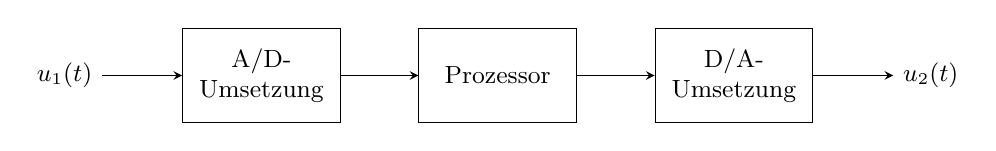
\begin{tikzpicture}[>=stealth, font=\small]
  \node at (0,0) (in) {$u_1(t)$};
  \node[draw, rectangle, minimum width=2cm, minimum height=1.2cm, align=center] at (2.5,0) (ad) {A/D-\\Umsetzung};
  \node[draw, rectangle, minimum width=2cm, minimum height=1.2cm, align=center] at (5.5,0) (proc) {Prozessor};
  \node[draw, rectangle, minimum width=2cm, minimum height=1.2cm, align=center] at (8.5,0) (da) {D/A-\\Umsetzung};
  \node at (11,0) (out) {$u_2(t)$};
  \draw[->] (in) -- (ad);
  \draw[->] (ad) -- (proc);
  \draw[->] (proc) -- (da);
  \draw[->] (da) -- (out);
\end{tikzpicture}
\end{center}

\section{Analog-Digital-Umsetzung}

Die A/D-Umsetzung beinhaltet drei wesentliche Schritte:
\begin{itemize}
  \item Abtastung des zeitkontinuierlichen Signals
  \item Quantisierung der abgetasteten Signalwerte
  \item Umsetzung der quantisierten Werte in einen digitalen Code
\end{itemize}

\begin{itemize}
  \item Abtastung unter bestimmten Bedingungen ohne Informationsverlust
  \item Quantisierung in der Regel mit Informationsverlust
\end{itemize}

\section{Abtastung}

Entnahme von „Signalproben" in regelmäßigen Intervallen. Definition einer Abtastfrequenz oder Abtastrate $f_A$:

$$
f_A = \frac{\text{Zahl der Abtastwerte}}{\text{Zeiteinheit}}
$$

Typische Abtastraten:
\begin{itemize}
  \item Telefonsprache (ISDN, GSM, UMTS) \hfill 8\,kHz, 16\,kHz
  \item Audio-CD \hfill 44{,}1\,kHz
  \item DAT-Rekorder \hfill 48\,kHz
\end{itemize}

\subsection*{Abtastung des Sinussignals}

Das analoge Signal $x(t)$ wird in regelmäßigen Abständen $T_A$ abgetastet, woraus die diskrete Folge $x[k] = x(kT_A)$ entsteht.

\subsection*{Rekonstruktion des analogen Signals}

Aus den Abtastwerten lässt sich das analoge Signal näherungsweise rekonstruieren. Zwei gängige Methoden sind:
\begin{itemize}
  \item \textbf{Interpolation 0-ter Ordnung:} Jeder Abtastwert wird bis zum nächsten Abtastzeitpunkt konstant gehalten (Treppenform).
  \item \textbf{Lineare Interpolation:} Aufeinanderfolgende Abtastwerte werden durch Geraden verbunden.
\end{itemize}

\subsection*{(Ideale) Rekonstruktion mit si-Funktionen}

Die ideale Rekonstruktion des analogen Signals aus seinen Abtastwerten erfolgt durch Überlagerung von si-Funktionen, eine pro Abtastwert:

$$
\hat{x}(t) = \sum_{k=-\infty}^{\infty} x[k]\, \operatorname{si}\!\left(\frac{t - kT_A}{T_A}\right)
$$

Beispiel: $f = \dfrac{1}{T}$, $f_A = \dfrac{5}{T} = 5f$.

\subsection*{Spektrogramme}

Das Spektrogramm des Originalsignals und des nach Interpolation 0.\ Ordnung rekonstruierten Signals zeigen deutliche Unterschiede im Hochfrequenzbereich. Lineare Interpolation und Interpolation mit si-Funktionen liefern eine deutlich bessere Annäherung an das Originalsignal.

\subsection*{Ist die Rekonstruktion eindeutig?}

Die Rekonstruktion ist nur dann eindeutig, wenn die Abtastwerte das Signal vollständig beschreiben. Dabei gilt:

$$
\Rightarrow \text{Die Nullstellen der si-Funktion müssen im Raster } 1/f_A \text{ liegen!}
$$

\subsection*{Wie viele Abtastwerte sind erforderlich?}

Bei einer Abtastrate von $f_A = \dfrac{5}{2T}$ ist eine eindeutige Rekonstruktion des Signals möglich.

Bei einer Abtastrate von $f_A \approx \dfrac{4}{2T}$ (mit $\tilde{T} = 4T$) gelingt die Rekonstruktion ebenfalls noch fehlerfrei.

Offenbar geht im letzten Fall \textit{bei der Abtastung} die Information über die wahre Signalfrequenz verloren.

Die Rekonstruktion mit si-Funktionen liefert in diesem Fall ein Sinussignal bei einer tieferen Frequenz

$$
\tilde{f} = f_A - f,
$$

wobei $\tilde{f}$ die sogenannte \textit{Spiegelfrequenz} darstellt. Der oben beschriebene Effekt wird in der englischen Literatur häufig als \textit{aliasing} bezeichnet.

\section{Das Abtasttheorem}

Die in einem Signal enthaltene maximale Frequenz bestimmt die erforderliche Anzahl von Abtastwerten pro Zeiteinheit. Wenn die maximale Frequenz als Grenzfrequenz $f_g$ gegeben ist, muss also

$$
f_A > 2f_g
$$

gelten. Dieser Zusammenhang wird als \textit{Abtasttheorem} nach Nyquist oder Shannon bezeichnet. Die Abtastwerte werden dann in zeitlichen Intervallen $T_A = 1/f_A$ dem Signal entnommen und mit $x(kT_A)$, $k \in \mathbb{Z}$, bezeichnet.

\section{Quantisierung}

Die Amplitude $x(kT_A)$ eines Signalabtastwertes zum Zeitpunkt $t = kT_A$, $k \in \mathbb{Z}$, wird auf eine Menge endlicher, meist fest vorgegebener Werte, den Quantisierungsniveaus, abgebildet. Damit geht in der Regel ein Informationsverlust einher. Wird der quantisierte Wert mit $x_q(kT_A)$ bezeichnet, so kann der \textit{Quantisierungsfehler} des $k$-ten Abtastwertes mit

$$
\epsilon(kT_A) = x(kT_A) - x_q(kT_A)
$$

angegeben werden.

\section{Die Quantisierungskennlinie}

Der Zusammenhang zwischen zu quantisierenden und quantisiertem Wert kann mittels einer \textit{Quantisierungskennlinie} beschrieben werden.

Der (gleichmäßige) Quantisierer ist durch den Aussteuerbereich $[x_{\min}, x_{\max}]$ und die Stufenhöhe $\Delta x$ gekennzeichnet. Im obigen Beispiel gilt $x_{\min} = -1$, $x_{\max} = 1$ und $\Delta x = 0{,}25$.

\section{Der Quantisierungsfehler}

Der Quantisierungsfehler ist durch die Quantisierungsstufenhöhe beschränkt. Zur Berechnung der Quantisierungsfehlerleistung betrachten wir das folgende spezielle Eingangssignal (Rampe): Der Fehler $\epsilon(t) = x(t) - x_q(t)$ hat Sägezahnform mit Amplitude $\pm\tfrac{\Delta x}{2}$.

Bei einer großen Zahl von Quantisierungsstufen hat der Quantisierungsfehler rauschartigen Charakter. Beispiel einer Quantisierung mit $2^4 = 16$ Stufen:

Beispiel einer Quantisierung mit $2^{12} = 4096$ Stufen: Der Fehler $\epsilon(t)$ ist deutlich kleiner und kaum sichtbar.

\section{Dezibel}

\begin{itemize}
  \item Die Einheit Bel zeigt an, dass es sich um eine logarithmierte Verhältnisgröße handelt. Die Definition bezieht sich auf das Verhältnis zweier Leistungen $P_2$ und $P_1$:
  $$
  P = \log_{10}\!\left(\frac{P_2}{P_1}\right) \text{ [Bel]}
    = 10\log_{10}\!\left(\frac{P_2}{P_1}\right) \text{ [Dezibel]}
    = 10\,\text{lg}\!\left(\frac{P_2}{P_1}\right) \text{ [dB]}
  $$
  \item Beispiel: Die Leistung des Nutzsignals wird zur Rauschleistung ins Verhältnis gesetzt. Da das Ergebnis, der Signal-zu-Störabstand oder SNR (\textit{signal-to-noise ratio}), je nach Anzahl der Quantisierungsstufen über mehrere Größenordnungen variieren kann, ist es üblich, die Verhältnisgröße zu logarithmieren.
\end{itemize}

\subsection*{Einige dB-Werte}

\begin{center}
\begin{tabular}{cc|cc}
\toprule
\multicolumn{2}{c|}{\textbf{Leistungen}} & \multicolumn{2}{c}{\textbf{Amplituden}} \\
$\dfrac{P_2}{P_1}$ & $10\lg\!\left(\dfrac{P_2}{P_1}\right)$/dB
& $\dfrac{A_2}{A_1}$ & $20\lg\!\left(\dfrac{A_2}{A_1}\right)$/dB \\
\midrule
0{,}01      & $-20$ & 0{,}01      & $-40$ \\
0{,}1       & $-10$ & 0{,}1       & $-20$ \\
0{,}25      & $-6$  & 0{,}25      & $-12$ \\
0{,}5       & $-3$  & 0{,}5       & $-6$  \\
$1/\sqrt{2}$& $-1{,}5$ & $1/\sqrt{2}$ & $-3$ \\
1           & $0$   & 1           & $0$   \\
$\sqrt{2}$  & $1{,}5$  & $\sqrt{2}$   & $3$  \\
2           & $3$   & 2           & $6$   \\
4           & $6$   & 4           & $12$  \\
10          & $10$  & 10          & $20$  \\
100         & $20$  & 100         & $40$  \\
\bottomrule
\end{tabular}
\end{center}

\subsection*{Quantisierung eines Bildsignals}

$\Rightarrow$ Die Qualität des rekonstruierten Signals hängt wesentlich von der Zahl der Quantisierungsniveaus ab.

\section{Codierung: Natürliche binäre Zahlen}

\begin{center}
\begin{tabular}{lcc}
\toprule
\textbf{Menge} & \textbf{Dezimale Zahl} & \textbf{Natürliche binäre Zahl} \\
\midrule
       & 0 & 0    \\
$\bullet$     & 1 & 1    \\
$\bullet\bullet$    & 2 & 10   \\
$\bullet\bullet\bullet$   & 3 & 11   \\
$\bullet\bullet\bullet\bullet$  & 4 & 100  \\
$\bullet\bullet\bullet\bullet\bullet$ & 5 & 101  \\
$\bullet\bullet\bullet\bullet\bullet\bullet$ & 6 & 110  \\
$\bullet\bullet\bullet\bullet\bullet\bullet\bullet$ & 7 & 111  \\
$\bullet\bullet\bullet\bullet\bullet\bullet\bullet\bullet$ & 8 & 1000 \\
\bottomrule
\end{tabular}
\end{center}

\section{Prinzip der Codierung}

Die Quantisierungsniveaus eines Quantisierers lassen sich durch einen binären Code mit endlich vielen Stellen repräsentieren.

Bei binärer Codierung ergibt sich aus der Wortbreite $w$ die Zahl darstellbarer Quantisierungsstufen zu $2^w$.

\subsection*{Typische Wortbreiten}

\begin{center}
\begin{tabular}{lcc}
\toprule
\textbf{Signal} & \textbf{Wortbreite $w$} & \textbf{Anzahl der Quantisierungsniveaus} \\
\midrule
Sprache & 8--16 Bit      & 256 -- 65\,536         \\
Audio   & 16--24 Bit     & 65\,536 -- 16\,777\,216 \\
Video   & $3 \times 8$ Bit & $3 \times 256$         \\
\bottomrule
\end{tabular}
\end{center}

\section*{Zusammenfassung}

\begin{itemize}
  \item Informationstragende Signale entstehen auf vielfältige Weise. Es werden analoge, zeitdiskrete, wertdiskrete und digitale Signale unterschieden.
  \item Sie lassen sich häufig als Summe elementarer Signale darstellen.
  \item Die digitale Verarbeitung analoger Signale erfordert eine Abtastung, Quantisierung und Codierung.
  \item Die Abtastung ist verlustfrei, wenn das Abtasttheorem eingehalten wird.
  \item Die Quantisierung führt in der Regel zu einem Informationsverlust.
\end{itemize}